\section{CanOp}
\label{sec_CanOp}
CanOp est le nom qui a été donné au projet de crée un équipement nouvelle génération pour la mine Somaïr au Niger. Cette sonde est composée de 3~éléments majeurs.
\begin{itemize}
    \item 2 Sondes de rayonnement Gamma fournissent par la société Geovista
    \item une partie électronique qui inclue l'alimentation par batterie. %geovista
    \item Un GPS différentiel fourni par Ophelia
\end{itemize}
Un opérateur utilise cette sonde en connexion avec une tablette pour déterminer ou extraire du minerai.%figure de la canop
\subsection{Les sondes Gamma}
\label{ssec_sonde}



Les sondes gamma de cet appareil proviennent de chez Geovista et sont composées de deux parties.

\begin{figure}

    \begin{subfigure}{1\textwidth}
        \centering
        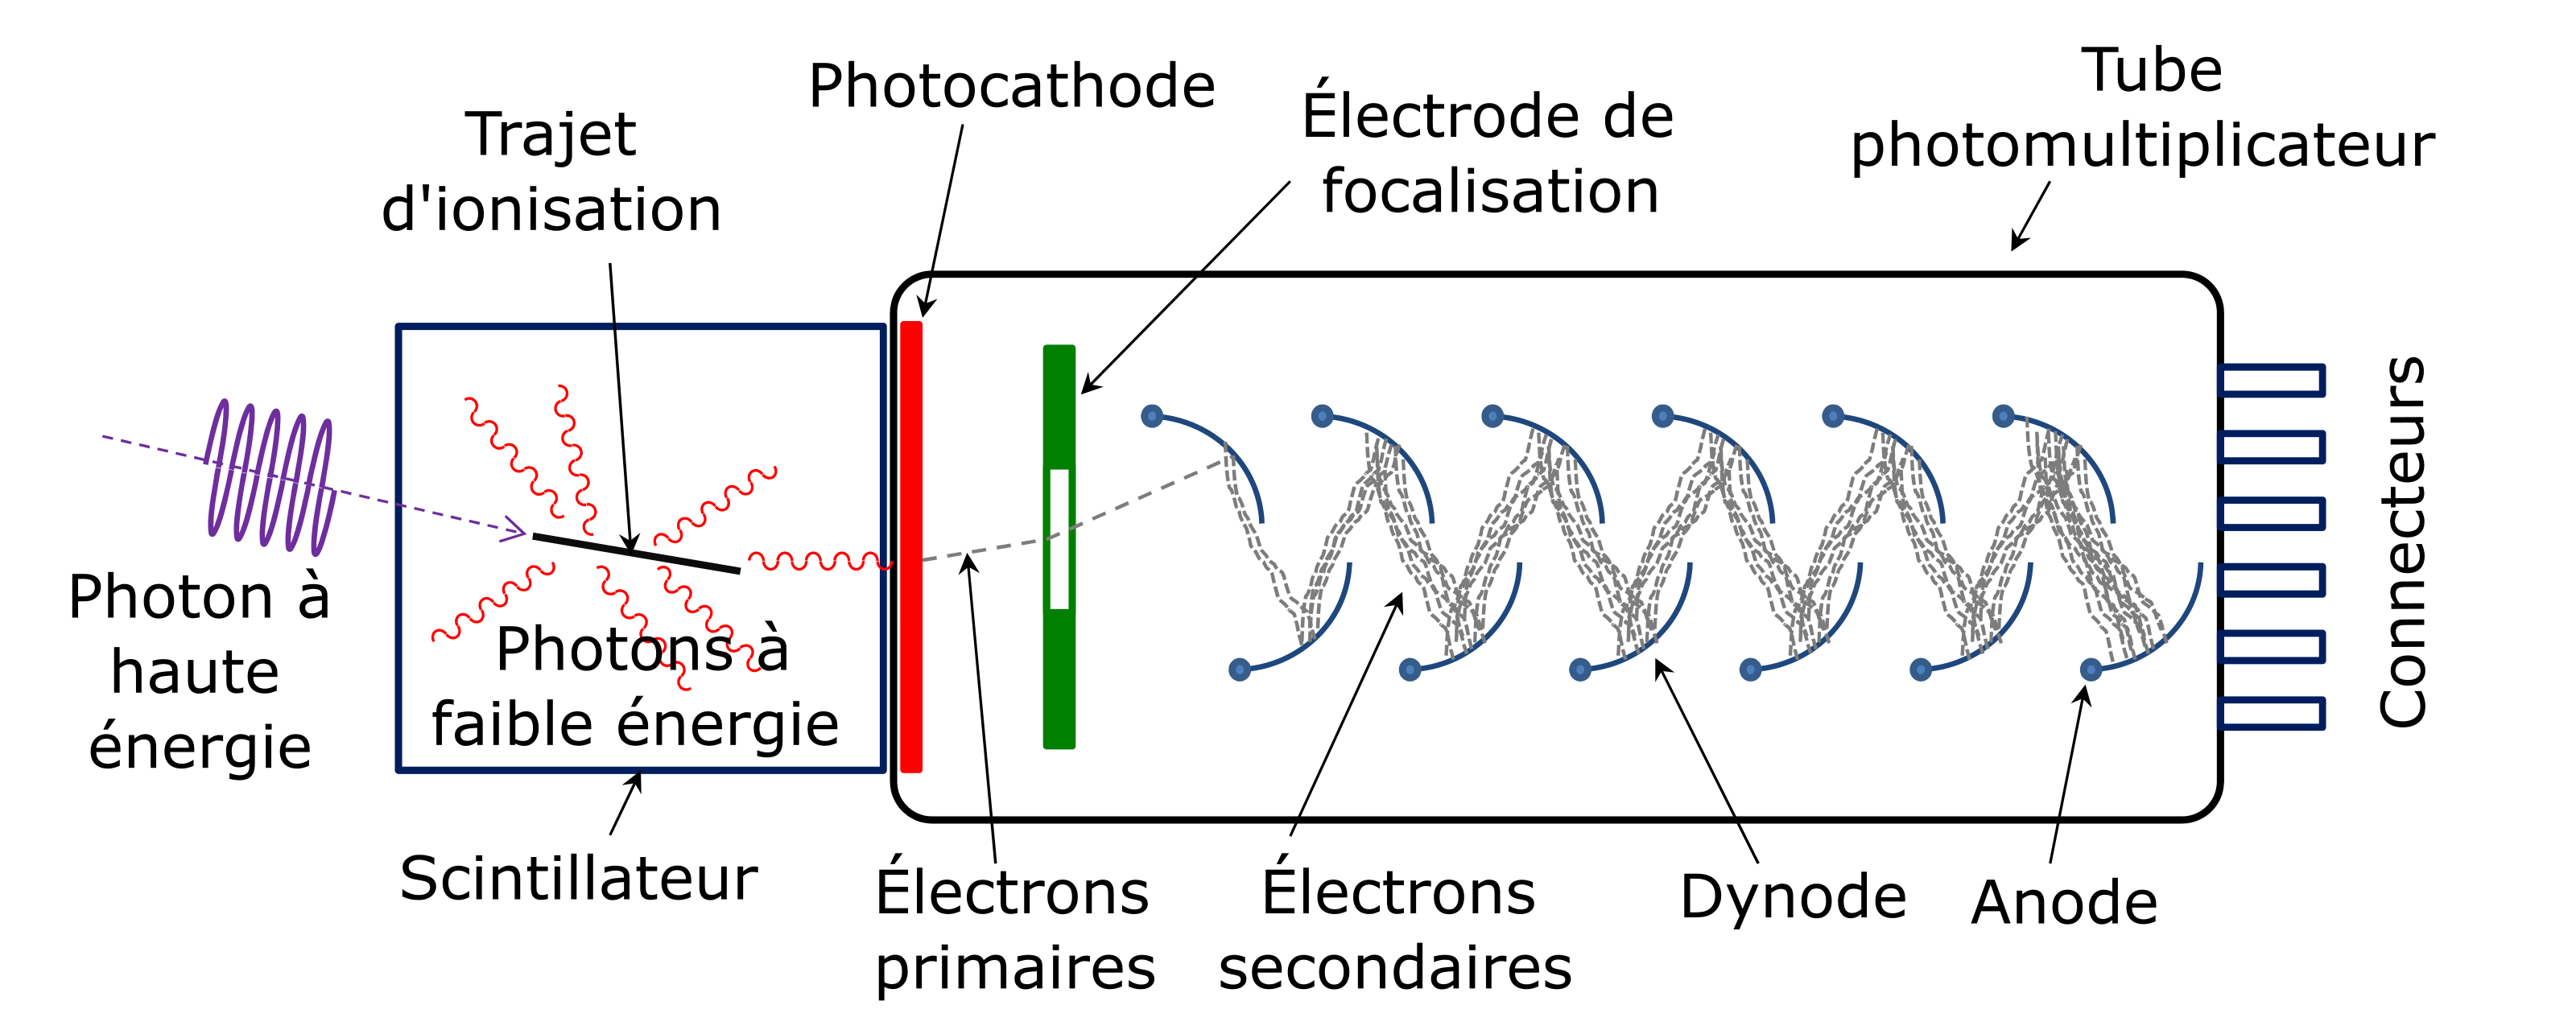
\includegraphics[width=1\textwidth]{she/Photomultiplier_coupled_to_a_scintillator_-_fr.png}
        \caption[Shema d'une sonde gamma NaI]{Schéma d'une sonde gamma NaI. Source~: \href{https://commons.wikimedia.org/wiki/File:Photomultiplier_coupled_to_a_scintillator_-_fr.png}{Qwerty123uiop}, \href{https://creativecommons.org/licenses/by-sa/3.0}{CC BY-SA~3.0}, via Wikimedia Commons}
        \label{fig_detecteur_gamma}
    \end{subfigure}
    \begin{subfigure}[t]{0.32\textwidth}
        \centering
        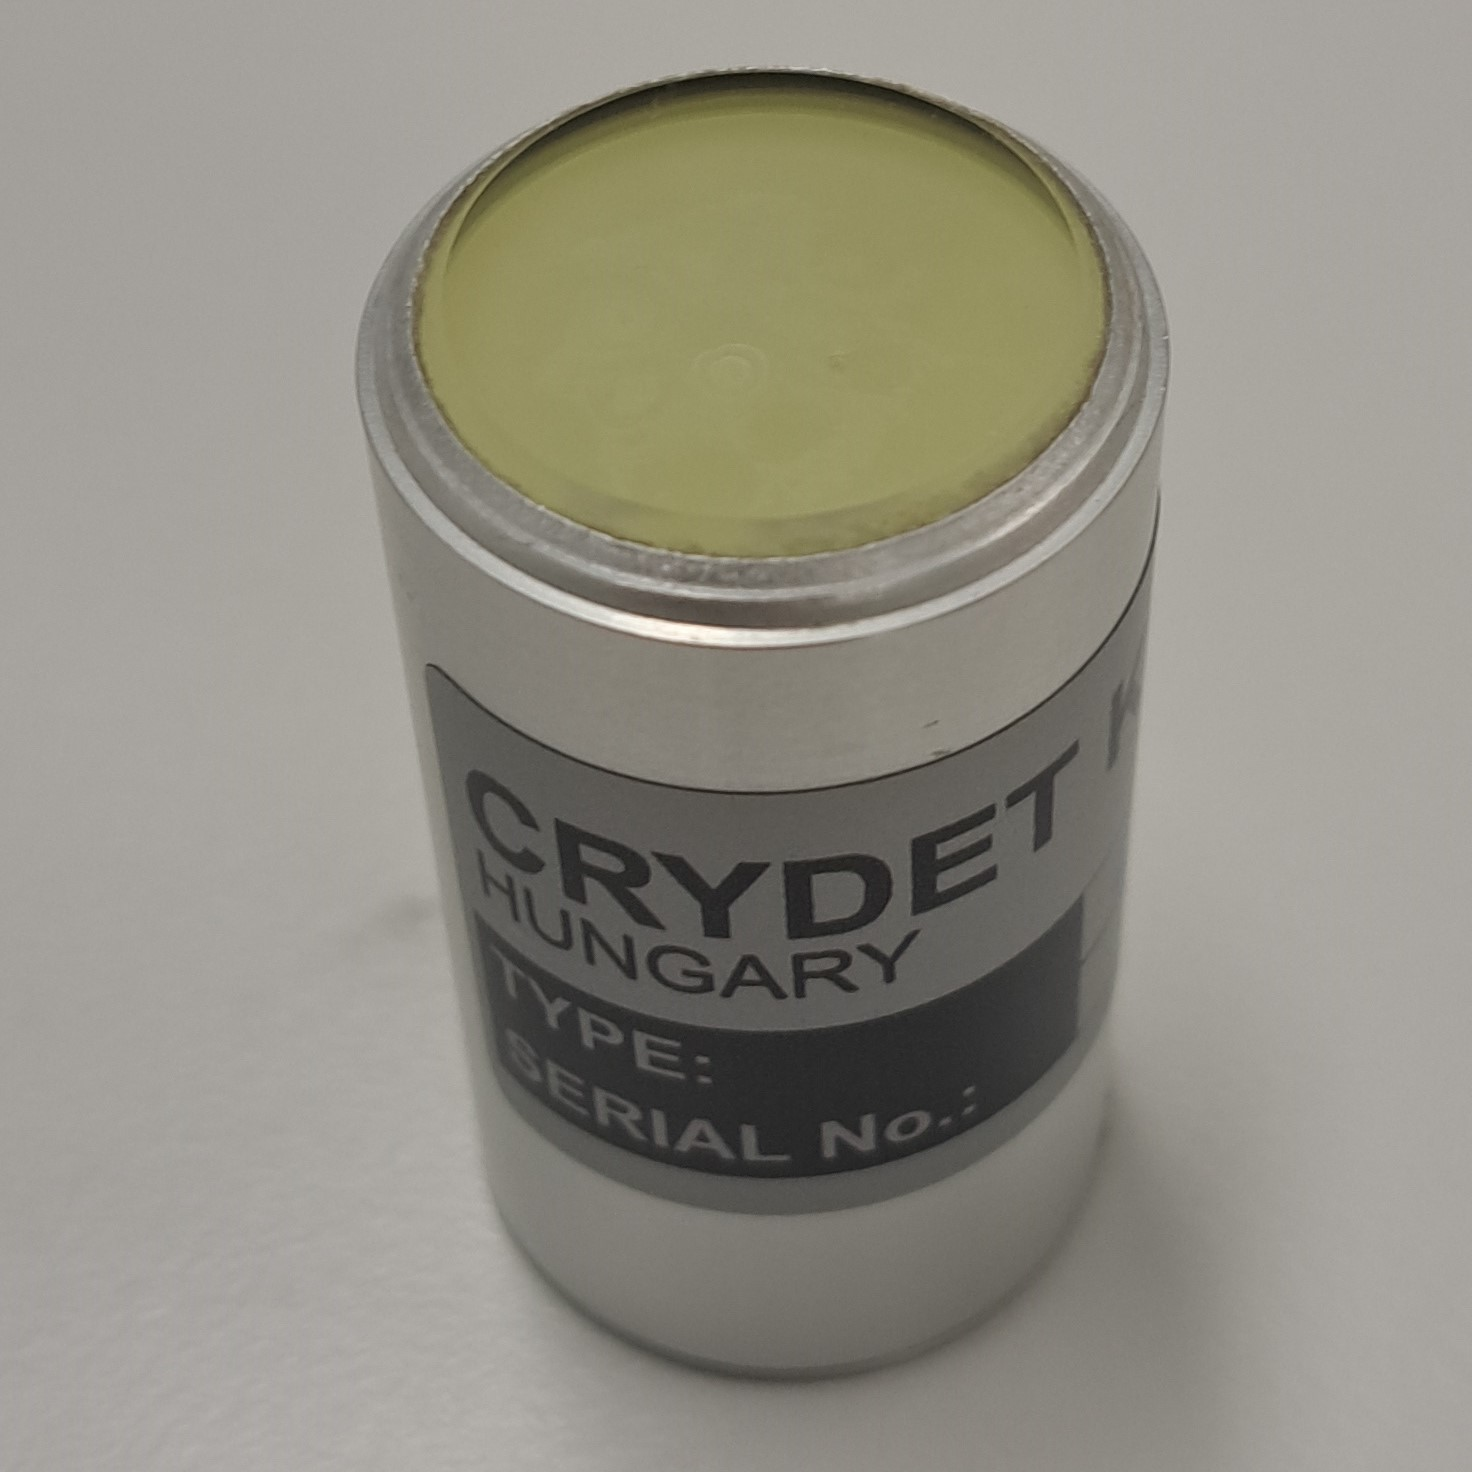
\includegraphics[width=0.9\textwidth]{photo/Crystal.jpg}

        \caption[Photo d'un cristal NaI]{Photo d'un cristal NaI doper au thallium. Dimension~: diamètre 28*50~mm}
        \label{fig_Nai}
    \end{subfigure}
    \begin{subfigure}[t]{0.32\textwidth}
        \centering
        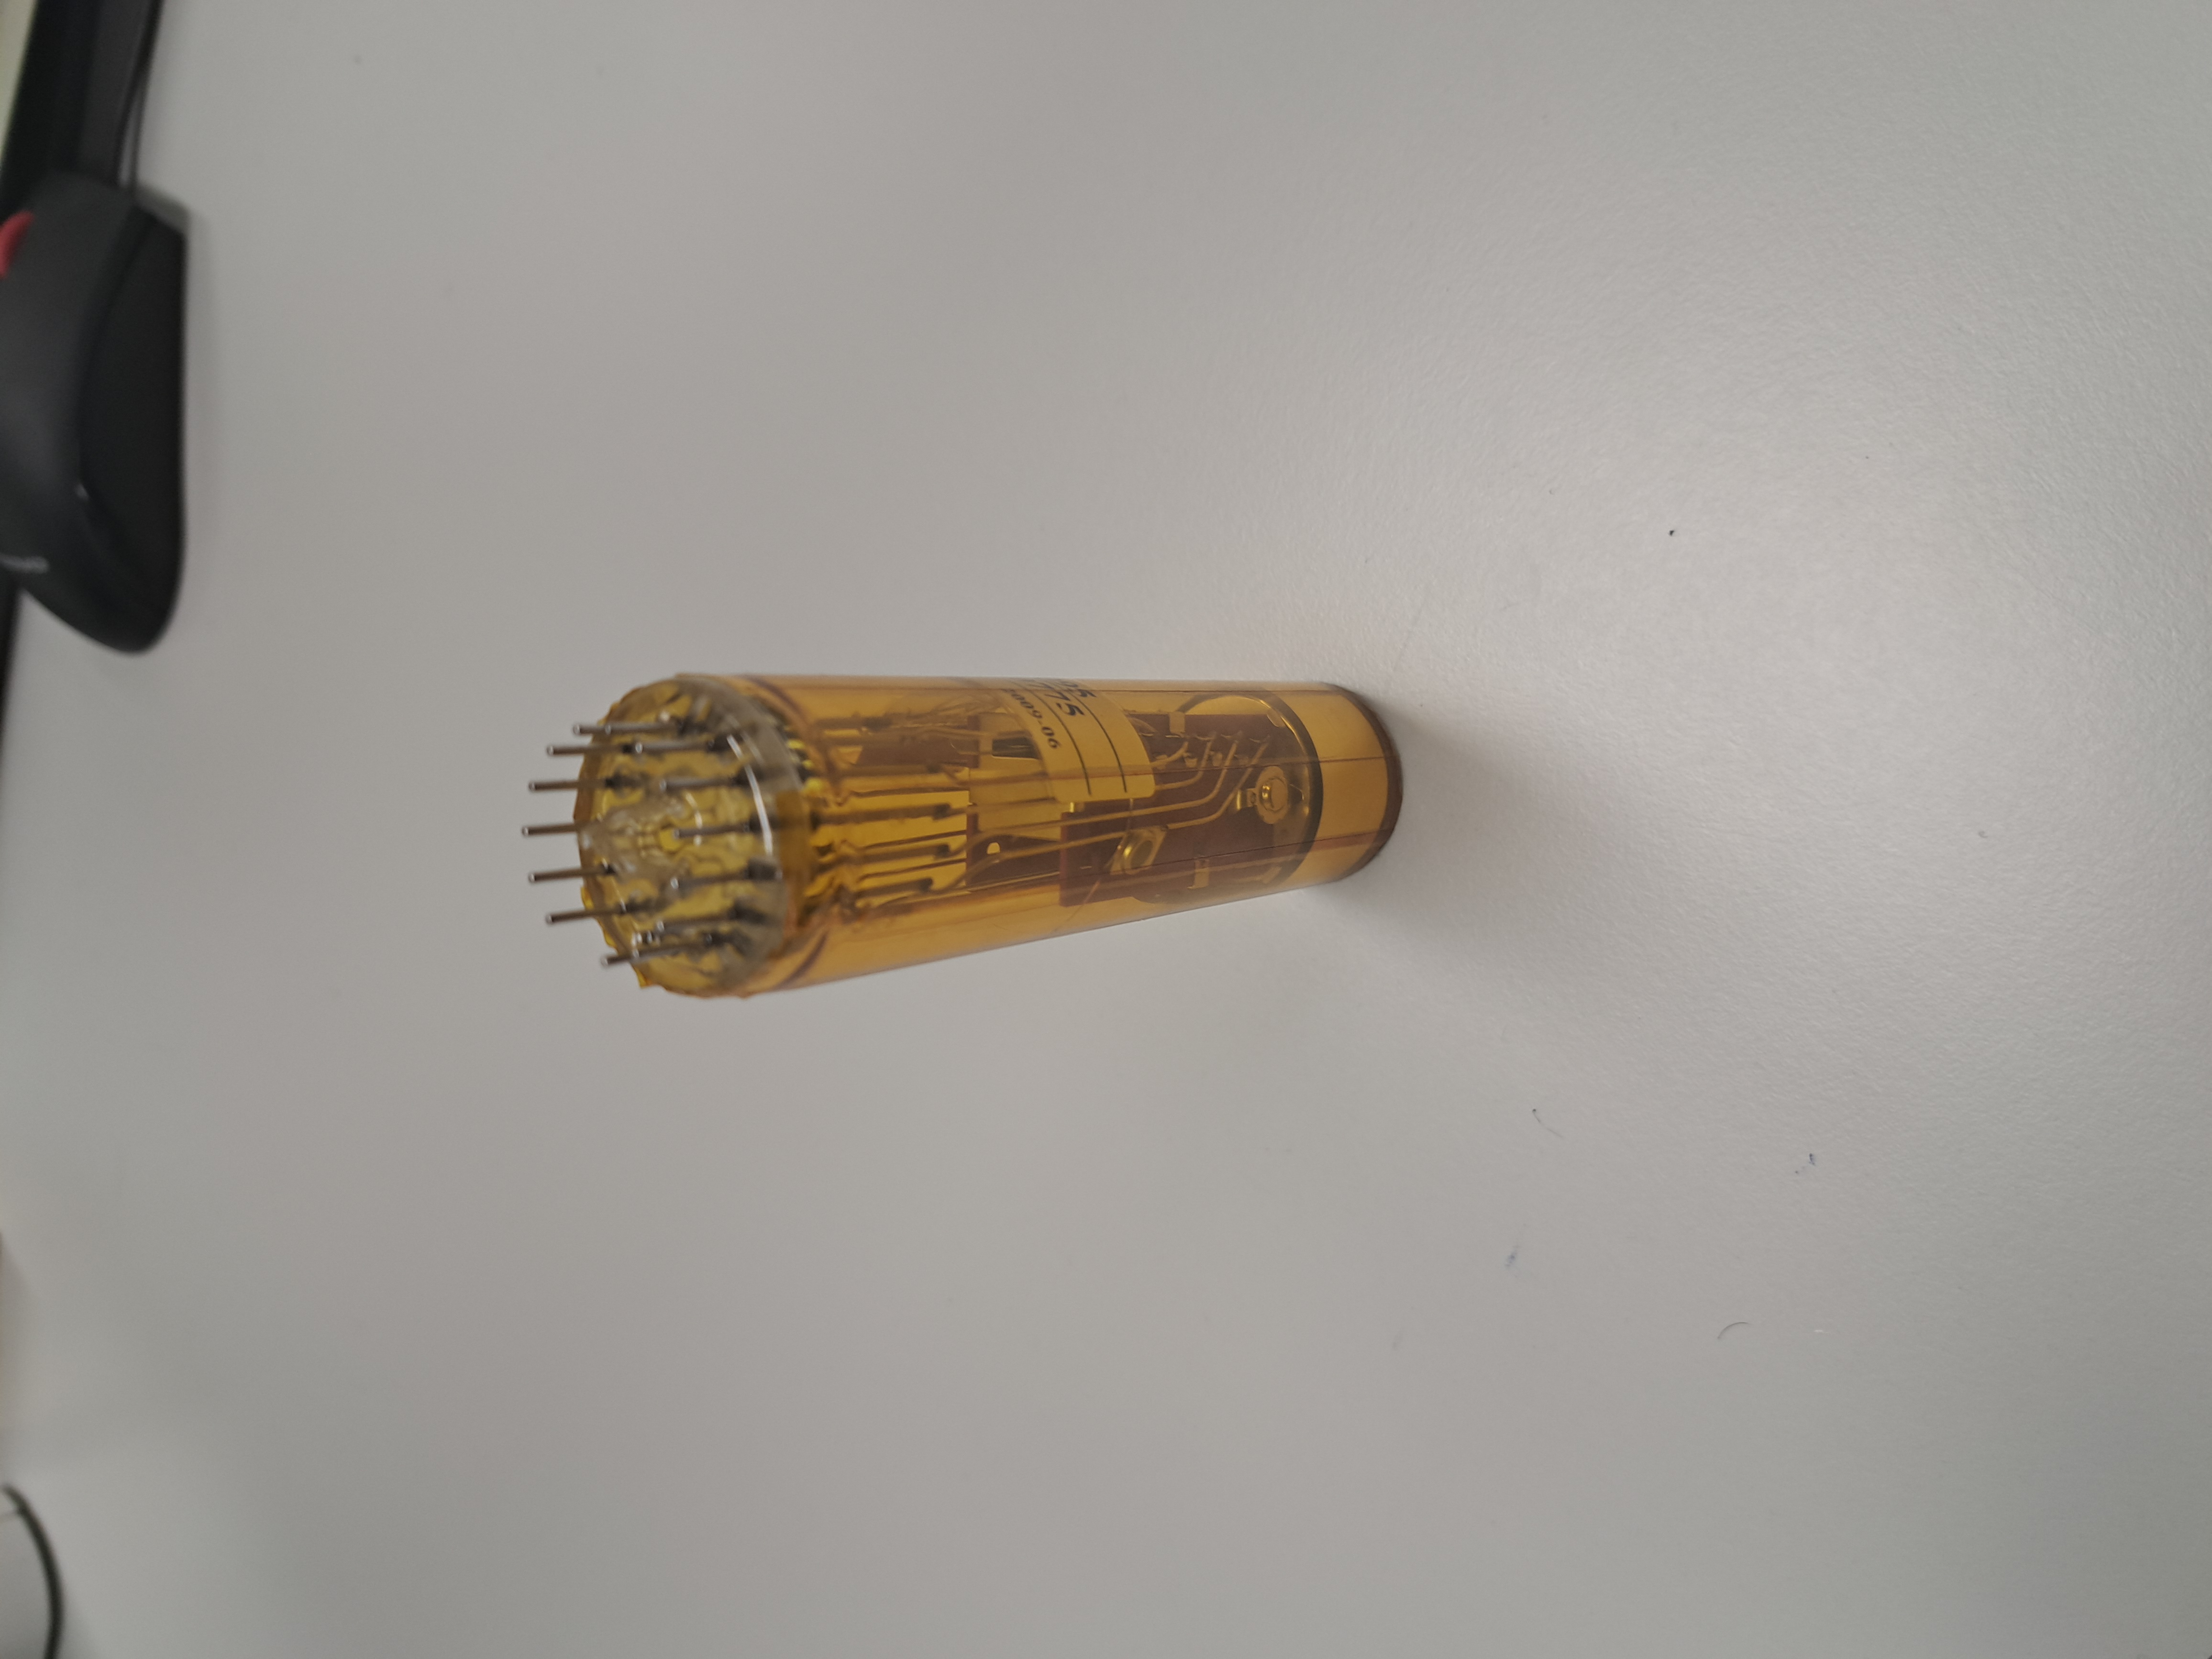
\includegraphics[width=0.9\textwidth]{photo/PMT.jpg}

        \caption[Photo d'un tube photomultiplicateur]{Photo d'un tube photomultiplicateur. Noter la fêlure à gauche de l'étiquette. Dimension~: diamètre 29*114~mm}
        \label{fig_PMT}
    \end{subfigure}
    \begin{subfigure}[t]{0.32\textwidth}
        \centering
        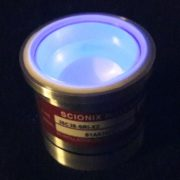
\includegraphics[width=0.9\textwidth]{photo/cristal_glow.jpg}
        \caption[Photo d'un cristal NaI en scintillation]{Photo d'un cristal NaI en scintillation. Le pic d'émission du cristal est à 430~nm Source~: scionix.}
    \end{subfigure}
    \caption{Fonctionnement d'une sonde gamma à scintillation}

\end{figure}

\newpage

\begin{wrapfigure}{r}{0.4\textwidth}
    \centering
    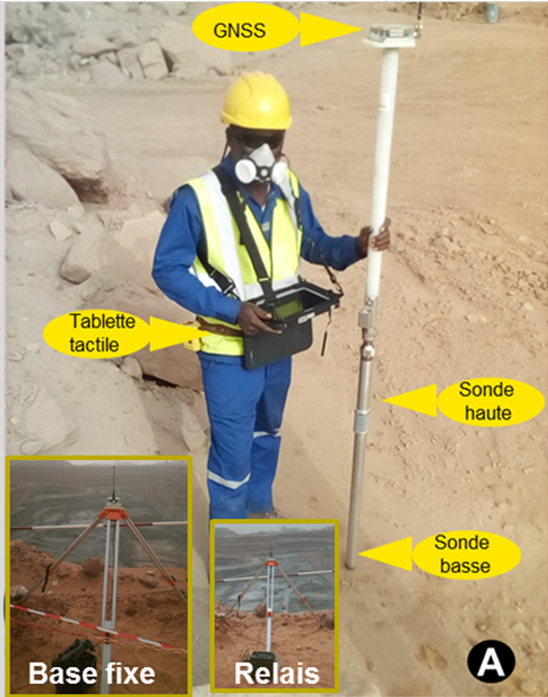
\includegraphics[width=0.4\textwidth]{photo/ap_avec_canop.png}
    \caption{Photo d'un aide-prospecteur tenant la CanOP}
\end{wrapfigure}

\begin{description}
    \item[Un cristal NaI(Th)] C'est un cristal formé de sodium et d'iode avec quelque atome de thallium reparti dans sa structure cristalline. Quand un photon vient frapper un atome du cristal il va devenir ioniser due a la grand énergie du photon. En se de-excitant, les atomes doivent repasser par des niveaux d'énergie et donc l'énergie qu'il dissipe à travers une émission de photon doit avoir une énergie précis qui ce traduit par une longueur d'onde dans le visible. Nous avons donc un outil capable de transformer un rayonnement haut en énergie en quelque chose avec moins d'énergie que nous savons mesurer. (voir partie gauche de la \cref{fig_detecteur_gamma,fig_Nai})~\cite{site:explication_NaI}
    \item[Un tube photomultiplicateur]ce tube permet de convertir un photon en un photoélectron qui est ensuite multiplié par le tube pour être converti en signaux électriques. Pour cela quand un photon vient du cristal NaI, il impact une photocathode qui éject un électron dû à l'effet photoélectrique. Les électrons résultants sont ensuite accélérés vers la première dynode, car elle a un potentiel $\sim$~100~V. Comme il accélère, il gagne de l'énergie et quand il frappe la dynode, elle va relâcher plusieurs électrons de plus basse énergie. Ces photons vont si ensuit être accéléré par le prochain échelon qui est lui aussi tenu a un potentielle de $\sim$~100~V par rapport a l'étape d'avant. Si chaque échelon multiplie par 4 et qu'il y a 12~étapes, notre gain serait de $4^{12}\approx10^{7}$. L'utilisation d'un PMT implique d'avoir un générateur de haute tension, car la photocathode sera maintenue a $\sim-1200$~V, il faut une atmosphère protectrice ou que le vide soit fait dans le tube et qu'il soit protéger de champs magnétiques, car il pourrait dévier les élections des dynode et ainsi réduire le gain du tube. (Voir partie droite de la \cref{fig_detecteur_gamma,fig_PMT})~\cite{book:photomultiplier_tube}
\end{description}

À la demande du client (Somaïr), une sonde basse a été incluse dans le projet en plus de la sonde haute prévue initialement pour permettre de faire des mesures au niveau du sol comme elle était faite avant (voir \cref{ssec_extraction,fig_AP_geiger}).
Les études internes montrent que les mesures les plus fiables sont faites à partir de la sonde haute donc la décision a été prise d'inclure les deux. À l'heure actuelle, selon les données enregistrées par la sonde, 68,5~\% des mesures sont faits à partir de la sonde haute et 29~\% à partir de la sonde basse. Les autres mesures sont faites avec une combinaison des deux.%parler de la sonde haut et du colimatage %figure des differente sonde

\subsection{Le GPS différentiel}
\label{ssec_Gps_differenciel}
Pour que la CanOp puisse fonctionner correctement, il faut qu'elle soit située très précisément ($\pm$ 10~cm sur les axes x et y et $\pm$ 1~cm sur les axes z), or un GPS classique n'arrive qu’a atteindre $\pm$~3~m horizontalement et $\pm$~5~m verticalement \cite{GPS_accuracy} dus notamment aux perturbations atmosphériques que subisse les signaux. %point de meure gamme doit etre precis
\begin{figure}[t]

    \begin{subfigure}[t]{0.5\textwidth}
        \centering
        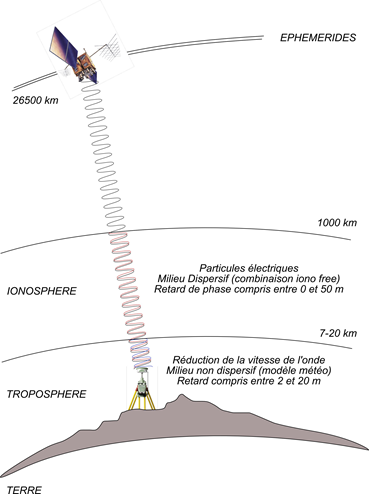
\includegraphics[height=0.9\textwidth]{she/GPS-mode-Naturel-5-10m.png}

        \caption[Source d'erreur des GPS]{Schéma présentant les sources d'erreur des GPS. Source~: Orphéon}
        \label{fig_GPS_error_source}
    \end{subfigure}
    \begin{subfigure}[t]{0.5\textwidth}
        \centering
        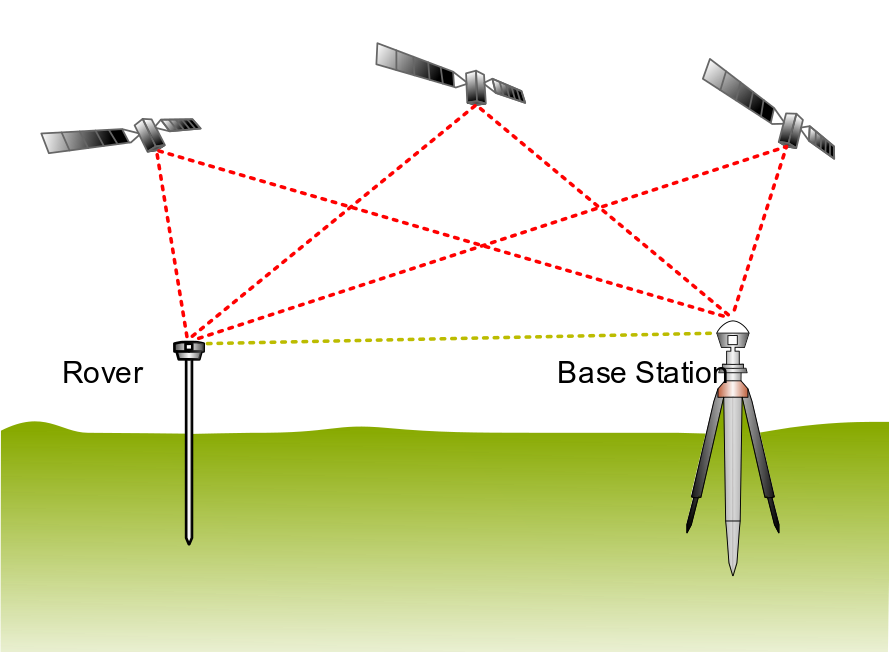
\includegraphics[width=0.9\textwidth]{she/Real_time_kinematic.png}

        \caption[Shema d'un systeme GPS differenciel]{Schéma d'un système GPS différentiel. Source~: \href{https://commons.wikimedia.org/wiki/File:Real_time_kinematic.svg}{TS Eriksson}, \href{https://creativecommons.org/licenses/by-sa/4.0}{CC BY-SA~4.0}, via Wikimedia Commons}
        \label{fig_RTK}
    \end{subfigure}
    \caption{Erreur du GPS et fonctionnement GPS RTK}
\end{figure}

Une des solutions possibles pour contourner ces problèmes est d'utiliser un GPS différentiel. Le principe de fonctionnement est $ sim$ple, une station fixe à proximité de notre zone de mesure reçoit également les signaux GPS et en connaissant sa position précise peuvent calculer et transmettre les corrections nécessaires. \cite{site:GPS_diff} %de la partie vers la partie modile

\subsection{L'électronique}

L'électronique de la CanOp est ce qui permet à tout de fonctionner ensemble. Cette électronique est composée de deux PCB~:
\begin{itemize}
    \item Un PCB pour la batterie et le bouton-poussoir
    \item Un PCB pour le GPS, les sondes et la communication Bluetooth avec la tablette
\end{itemize}

L'opérateur interagit avec avec la sonde que grâce à un bouton-poussoir qui peut lui donner du feed-back sur l'état de la sonde à travers deux LED intégré au bouton. Les données issues des sondes sont juste des pulses de courant que le second PCB convertit en signal numérique. C'est donner sont ensuite agrégé avec les donner du GPS qui sont transmis avec une connexion~RS-232. Les données sont ensuite renvoyées par ce bus au module du GPS qui contient le module Bluetooth qui permet de communiquer avec la tablette. Le GPS est connecté avec sont un connecteur 7~broches qui est multifonctions. Si l’on débranche le GPS, on peut utiliser ce connecteur pour charger la batterie interne de la sonde. Il existe également un dongle Bluetooth qui peut s’y connecter pour permettre l'interfaçage avec la sonde si le module GPS est indisponible. Les deux PCB sont contenus dans leur moitié de la sonde et sont interconnecté grâce à un connecteur 7~broches. Par mesure de sécurité, le fil positif de la batterie fait un aller-retour sur le connecteur entre les deux parties de la sonde pour que l'alimentation soit automatiquement coupée si l’on sépare les deux parties de la sonde.